% \documentclass[twoside,english,reqno,12pt,letters]{article}
\documentclass[a4paper,review,11pt,authoryear]{elsarticle}
% \journal{European Journal of Operational Research}
\journal{arXiv.org}
%\usepackage{kpfonts}
%\usepackage[utf8]{inputenc}
\usepackage{geometry}
\geometry{verbose,tmargin=1in,bmargin=1in,margin=1in,rmargin=1in}
\usepackage[labelsep=period]{caption}

%\usepackage[nolists,tablesfirst]{endfloat}
% \usepackage{babel}
\usepackage{array}
\usepackage{booktabs}
\usepackage{bm}
\usepackage{amsthm}
\usepackage{amsmath}
\usepackage{amstext}
\usepackage{graphicx}
\usepackage{natbib}
\usepackage{hyperref}
\usepackage{lineno}
\usepackage{bbm}
\usepackage{url}

\usepackage{algorithm}
\usepackage{algorithmicx}
\usepackage{algpseudocode}
\usepackage{verbatim}

\usepackage{setspace}
\linespread{1.5}

\usepackage{breakurl}
% \allowdisplaybreaks[1]

\usepackage{hyperref}
\hypersetup{
  colorlinks=true,
  linkcolor=blue,
  citecolor=blue,
  urlcolor=blue}

%% Fonts
\usepackage{bm}% Use \bm instead of \mathbf

%% Reduce Bibliography space
\usepackage{enumitem}
\setlength{\bibsep}{0.0pt}
\setlength{\itemsep}{0.0pt}

\newtheorem{theorem}{Theorem}
\newtheorem{lemma}[theorem]{Lemma}
\newtheorem{definition}{Definition}
\newtheorem{algthm}[theorem]{Algorithm}


\begin{document}

\begin{frontmatter}

  \title{}
  % \title{The uncertainty estimation of feature-based time series forecasts} % EJOR does not like acronyms

  % include affiliations in footnotes:


  \begin{abstract}

  \end{abstract}

  \begin{keyword}

  \end{keyword}

\end{frontmatter}

%% \linenumbers

\newpage
\setcounter{page}{1}


\section{Methodology}
\label{sec:method}

We proposed a novel approach based on linear combination of forecasting models (e.g., ETS, ARIMA, etc.), which is characterized by taking features into consideration. In the framework of our method, there are two process: training process and forecasting process. During training, a collection of time series to be predicted, a pool of forecasting models and a set of functions to compute features are necessary inputs, and coefficient vectors assessed by a log predictive scoring rule \citep{geweke2011optimal} are obtained for next forecasting process. In forecasting process, the weights of models are produced on the basis of features and coefficient vectors. From these, the linear combined forecasting results of each time series can be computed, which form outputs. The flowchart of proposed method for one time series is shown in Figure~\ref{fig:flowchart}. Multiple time series forecasting only need to repeat the above process. The pseudo-code of the proposed framework can be seen in Algorithm~\ref{alg:opt}.

The main innovative point of our method is to produce weights for all methods in the pool by transforming weights into functions of features. Thus, training the optimal weight of each method is to train the optimal coefficient vector of features for every model. The functions to calculate features are implemented in the tsfeatures R package by \cite{hyndman2018tsfeatures}. The objective of optimization is maximizing log predictive score function, where the predictive distributions are obtained by Bayesian approach. Relevant details are shown in Algorithm~\ref{alg:opt}.


\begin{figure}
  \centering 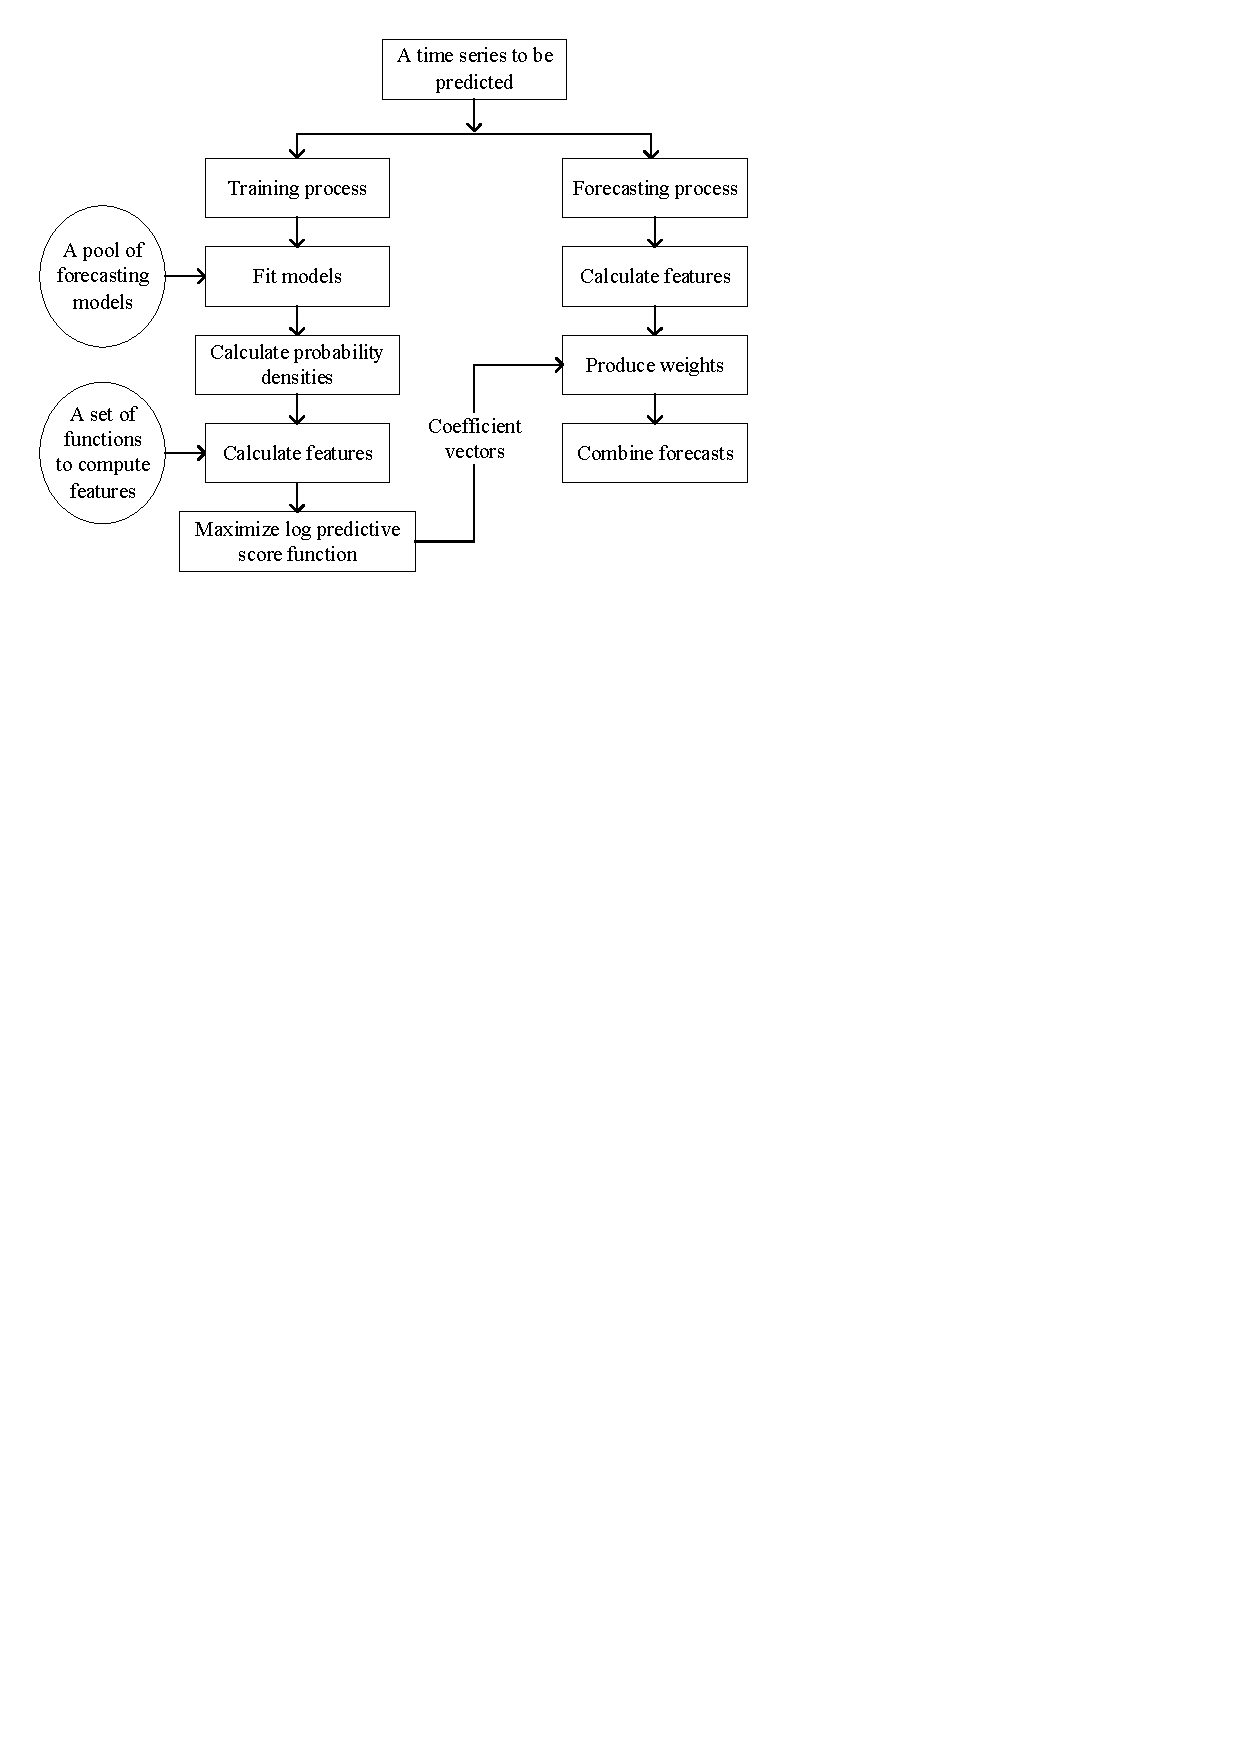
\includegraphics[width=0.7\textwidth]{figures/flowchart.pdf}
  \caption{Flowchart of the proposed method for one time series}
  \label{fig:flowchart}
\end{figure}

% Theoretically, schemes for generating combination weights should perform well on identifying poorly performing methods and on assigning a tiny weight to these methods. The necessity of the additional selection step would thus seem to depend on the number and performance of the benchmark forecasting methods and also on the scheme for computing weights, etc.

\begin{algorithm}
  \renewcommand{\algorithmicrequire}{\textbf{Input:}}
  \renewcommand{\algorithmicensure}{\textbf{Output:}}
  \caption{The framework of Bayesian model combination based on features}
  \label{alg:opt}
  \begin{algorithmic}
    \Require ~~\\
    $R=\left( {{Y}_{1}},{{Y}_{2}},\cdots ,{{Y}_{N}} \right)$: A collection of $N$ time series.\\
    $M=\left( {{M}_{1}},{{M}_{2}},\cdots ,{{M}_{m}} \right)$: $m$ forecasting models in the pool.\\
    $F$: a set of functions to compute time series’ features.
    \Ensure ~~\\
    $m-1$ coefficient vectors of features.\\
    Forecasting values.
  \end{algorithmic}
  \begin{algorithmic}[1]
  	\For{$n=1$ to $N$}\\
  	TRIANING PROCESS
  	\State Fit m forecasting models for the time series${{Y}_{n}}=\left\{ {{y}_{1}},{{y}_{2}},\cdots ,{{y}_{{{l}_{n}}}} \right\}$ , then the fitted values$\left\{ y{{f}_{1j}},y{{f}_{2j}},\cdots ,y{{f}_{{{l}_{n}}j}} \right\}$$\left( j=1,2,\cdots ,m \right)$ , the estimated residual variance $\sigma _{nj}^{2}$ and forecasts $\left\{ y{{f}_{1j}},y{{f}_{2j}},\cdots ,y{{f}_{{{h}_{n}}j}} \right\}$ are obtained.
  	\State Construct the probability density matrix ${{P}^{{{l}_{n}}*m}}$ , consist of
  	\[{{p}_{tj}}=p\left( y_{t}^{o};\widetilde{y}_{t-1}^{o},{{M}_{j}} \right),{{\widehat{y}}_{t}}\sim N\left( y{{f}_{tj}},\sigma _{nj}^{2} \right)\]
  	where $t=1,2,\cdots ,{{l}_{n}}$,$j=1,2,\cdots ,m$,‘‘o’’ for ‘‘observed’’, and $\widetilde{y}_{t-1}^{o}=\left\{ y_{1}^{o},y_{2}^{o},\cdots ,y_{t-1}^{o} \right\}$.
  	\For{$t=10$ to ${{l}_{n}}$}
  	\State Calculate the set of features of ${{Y}_{n}}$ using $F$ from starting date to time $t$, denoted ${{X}_{t+1}}$.
  	\EndFor
  	\State Train $m-1$ coefficient vectors ${{\beta }_{nj}}\left( j=1,2,\cdots ,m-1 \right)$ of features, by maximizing log predictive score function (since the features of historical data cannot be calculated when $t =1,...,9$, the weight was arbitrarily set at 0.5):
  	\[\underset{{{\beta }_{nj}}}{\mathop{\arg \max }}\,=\sum\limits_{t=1}^{9}{\log \left[ \frac{1}{m}\sum\limits_{j}^{m}{{{p}_{tj}}} \right]}+\sum\limits_{t=10}^{{{l}_{n}}}{\log \left[ \sum\limits_{j}^{m}{{{w}_{j}}{{p}_{tj}}} \right]}\]
  	\[{{w}_{1,2,\cdots ,m-1}}=\frac{1}{1+\exp \left\{ -{{X}_{t}}{{\beta }_{nj}} \right\}},{{w}_{m}}=1-\sum\limits_{j=1}^{m-1}{{{w}_{j}}}\]
  	FORECASTING PROCESS
  	\For{$i=1 $ to ${{h}_{n}}$}
  	\State Calculate the set of features from starting date to time ${{h}_{n}}+i-1$, denoted ${{X}_{{{l}_{n}}+i}}$.
  	\State Combine forecasts from $m$ models as follows:\\
  	\[{{\widehat{y}}_{{{l}_{n}}+i}}=\sum\limits_{j}^{m}{{{\omega }_{j}}y{{f}_{ij}}},\ {{\omega }_{1,2,\cdots ,m-1}}=\frac{1}{1+\exp \left\{ -{{X}_{{{l}_{n}}+i}}{{\beta }_{nj}} \right\}},\ {{\omega }_{m}}=1-\sum\limits_{j=1}^{m-1}{{{\omega }_{j}}}\]

  	\EndFor
  	\EndFor
  \end{algorithmic}

\end{algorithm}




% Table generated by Excel2LaTeX from sheet 'beta_correct'
\begin{table}[htbp]
	\centering
	\caption{The performance of different methods based on M4 quarterly data}
	\begin{tabular}{lrrr}
		\toprule
		\multicolumn{1}{c}{Method} & \multicolumn{1}{c}{Mase} & \multicolumn{1}{c}{Smape} & \multicolumn{1}{c}{Log score } \\
		\midrule
		\multicolumn{1}{p{22.445em}}{model combination with feature-based weights} & 1.111700 & 9.463586 & -89.805035 \\
		Feature-entropy (10) & 1.108626 & 9.401910 & -83.337199 \\
		Feature-seasonality (33) & 1.101129 & 9.342633 & -81.950126 \\
		Feature-alpha (16) & 1.107606 & 9.400229 & -83.985310 \\
		Feature-beta (17) & 1.102846 & 9.303098 & -82.331066 \\
		Feature-unitroot\_kpss (40) & 1.110846 & 9.420772 & -86.548085 \\
		Feature-arch\_acf (12) & 1.103709 & 9.307841 & -84.033347 \\
		Two features (17,33) & 1.109534 & 9.424416 & -85.307367 \\
		Three features (12,17,33) & \textbf{1.090470} & 9.284169 & -80.902124 \\
		Four features (10,12,17,33) & 1.103489 & 9.453321 & -82.783819 \\
		Five features (10,12,16,17,33) & 1.108070 & 9.404827 & -85.405179 \\
		Six features & 1.110544 & 9.426765 & -84.413829 \\
		\multicolumn{1}{p{22.445em}}{model combination with optimized weights} & 1.112378 & 9.455107 & -83.721742 \\
		\multicolumn{1}{p{22.445em}}{Simple average} & 1.090471 & \textbf{9.284165} & \textbf{-80.902121} \\
		ARIMA & 1.116552 & 9.569106 & -94.357188 \\
		ETS   & 1.115352 & 9.629163 & -86.376765 \\
		\bottomrule
	\end{tabular}%
	\label{tab:addlabel}%
\end{table}%


% Table generated by Excel2LaTeX from sheet 'beta0_correct'
\begin{table}[htbp]
	\centering
	\caption{The performance of different methods based on M4 quarterly data (intercept term included)}
	\begin{tabular}{lrrr}
		\toprule
		\multicolumn{1}{c}{Method} & \multicolumn{1}{c}{Mase} & \multicolumn{1}{c}{Smape} & \multicolumn{1}{c}{Log score } \\
		\midrule
		\multicolumn{1}{p{20.72em}}{model combination with feature-based weights } & 1.111702 & 9.461384 & -92.033372 \\
		Feature-entropy (10) & 1.107186 & 9.371883 & -83.634421 \\
		Feature-seasonality (33) & 1.108126 & 9.399961 & -83.790130 \\
		Feature-alpha (16) & 1.109946 & 9.429091 & -83.820810 \\
		Feature-beta (17) & 1.109957 & 9.439180 & -83.970490 \\
		Feature-unitroot\_kpss (40) & 1.110490 & 9.435423 & -84.094470 \\
		Feature-arch\_acf (12) & 1.110403 & 9.406790 & -84.039367 \\
		Two features (17,33) & 1.109328 & 9.427631 & -83.887800 \\
		Three features (12,17,33) & 1.109708 & 9.399365 & -85.131000 \\
		Four features (10,12,17,33) & 1.109713 & 9.398255 & -85.284220 \\
		Five features (10,12,16,17,33) & 1.108781 & 9.438102 & -84.648080 \\
		Six features & 1.114955 & 9.458814 & -86.604310 \\
		\multicolumn{1}{p{20.72em}}{model combination with optimized weights} & 1.112378 & 9.455107 & -83.721742 \\
		\multicolumn{1}{p{20.72em}}{Simple average} & \textbf{1.090471} & \textbf{9.284165} & \textbf{-80.902121} \\
		ARIMA & 1.116552 & 9.569106 & -94.357188 \\
		ETS   & 1.115352 & 9.629163 & -86.376765 \\
		\bottomrule
	\end{tabular}%
	\label{tab:addlabel}%
\end{table}%



%\section*{References}
\bibliographystyle{elsarticle-harv}
\biboptions{authoryear}
%\bibliography{full,References}
\bibliography{ref.bib}

%\newpage
% \appendix







\end{document}
